\documentclass[]{article}
\usepackage{lmodern}
\usepackage[margin=1in]{geometry}
\usepackage{setspace}
\usepackage{hyperref}
\usepackage{titlesec}
\usepackage{microtype}
\usepackage{tabularx}
\usepackage{graphicx}
\usepackage{booktabs}
\usepackage{amsmath, amssymb}

\renewcommand{\rmdefault}{phv} % Palatino

% --- Section numbering as 15-1, 15-2, ... ---
\renewcommand{\thesection}{15-\arabic{section}}
\setcounter{section}{0}


% --- Title ---
\title{Chapter 15: Instrumental Variables Estimation and Two-Stage Least Squares}
\author{}
\date{}


\begin{document}
\maketitle
 


% ----------------------
\section{Motivation: Omitted Variables in a Simple Regression Model}
 

\section*{1. Masalah Endogenitas}
Kita punya model:
\[
Y = \beta_0 + \beta_1 X + u, \quad \text{dengan } Cov(X,u)\neq 0
\]

Masalah: jika $x$ berkorelasi dengan error $u$ \; ($Cov(x,u) \neq 0$), maka \textbf{OLS bias} $\rightarrow$ tidak bisa dipercaya.
Dengan instrument variable, 
\[
X = \pi_0 + \pi_1 Z + v
\]
\section*{2. Syarat Instrumen}
Kita cari variabel baru $z$ (instrumen) untuk menggantikan variasi $x$ yang terkontaminasi error. Supaya $z$ sah jadi instrumen, harus memenuhi 2 syarat:

\begin{enumerate}
    \item \textbf{Eksogenitas instrumen}: 
    \[
    Cov(z,u) = 0 
    \]
    $\rightarrow$ instrumen tidak terkait dengan error.
    
    \item \textbf{Relevansi instrumen}: 
    \[
    Cov(z,x) \neq 0
    \]
    $\rightarrow$ instrumen cukup berkorelasi dengan variabel endogen.
Kalau dua syarat ini terpenuhi, $z$ bisa dipakai sebagai IV untuk $x$.

    \item \textbf{Syarat tambahan}: $Z$ hanya memengaruhi $Y$ lewat $X$, tidak lewat jalur lain, (sebenarnya bagian dari exogeneity - instrumen $Z$ tidak berkorelasi dengan error term.).
\end{enumerate}


\section*{3. Cara Mengecek}
\begin{itemize}
    \item Syarat (1) eksogenitas $\rightarrow$ sulit diuji langsung, biasanya berdasarkan argumen teori atau konteks.
    \item Syarat (2) relevansi $\rightarrow$ bisa diuji dengan regresi first stage:
    \[
    x = \pi_0 + \pi_1 z + v
    \]
    Kalau $\pi_1 \neq 0$, berarti $z$ relevan.
\end{itemize}

\section*{5. Estimator IV}
Kalau syarat terpenuhi, $\beta_1$ bisa diestimasi lewat:
\[
\beta_1 = \frac{Cov(z,y)}{Cov(z,x)}
\]

\noindent Versi sampel:
\[
\hat{\beta}_1 = \frac{\sum_{i=1}^{n} (z_i - \bar{z})(y_i - \bar{y})}{\sum_{i=1}^{n} (z_i - \bar{z})(x_i - \bar{x})}
\]

Artinya: IV pakai variasi $x$ yang “diprediksi” oleh $z$, bukan keseluruhan variasi $x$.


\section*{Inferensi Statistik dengan Estimator IV}

Dalam inferensi menggunakan IV (Instrumental Variables), varians asimptotik dari estimator IV bergantung pada kekuatan instrumen. Rumusnya menunjukkan bahwa varians IV adalah 
\[
\frac{\sigma^2}{n \sigma_x^2 \rho_{xz}^2},
\]
di mana $\rho_{xz}^2$ adalah kuadrat korelasi antara variabel endogen ($x$) dan instrumen ($z$). Hal ini berarti semakin lemah korelasi instrumen dengan variabel endogen, semakin besar varians IV estimator sehingga standard error meningkat. Dalam praktiknya, varians ini dihitung menggunakan residual dari regresi IV dan $R^2$ \textit{first stage}, sehingga ukuran kekuatan instrumen sangat menentukan presisi estimasi.

Dibandingkan dengan OLS, estimator IV selalu memiliki varians lebih besar, karena varians IV sama dengan varians OLS yang dibagi $R_{x,z}^2$, dan $R_{x,z}^2 < 1$. Artinya, IV kurang efisien dibanding OLS, terutama jika instrumen lemah. Namun, ketika variabel endogen berkorelasi dengan error, OLS menjadi bias dan tidak konsisten. Dalam situasi seperti ini, IV tetap lebih dapat dipercaya karena konsisten, meskipun kurang efisien. Dengan kata lain, pemilihan IV menekankan \textbf{konsistensi} daripada \textbf{efisiensi}.

\section*{Langkah Berpikir dalam Analisis IV}

\begin{tabularx}{\textwidth}{|c|X|X|}
\hline
\textbf{Langkah} & \textbf{Pertanyaan Kunci} & \textbf{Implikasi / Tindakan} \\
\hline
1. Tujuan Analisis & 
Apa hubungan kausal yang ingin diukur? \newline 
(misal: tambahan 1 tahun sekolah $\rightarrow$ naik berapa \% upah) & 
Tentukan variabel dependen ($Y$) dan variabel utama yang diminati ($X$). \\
\hline
2. Asumsi OLS & 
Apakah variabel utama ($X$) benar-benar eksogen? \newline 
(Cov($X,u$)=0) & 
Jika ya, OLS konsisten. Jika tidak, curiga endogenitas. \\
\hline
3. Identifikasi Endogenitas & 
Apakah ada faktor tak terukur yang memengaruhi $X$ dan $Y$ sekaligus? \newline 
(misal: ability, keluarga, motivasi) & 
Jika ada $\Rightarrow$ $X$ endogen $\Rightarrow$ OLS bias. \\
\hline
4. Solusi IV & 
Adakah variabel lain (instrumen) yang memengaruhi $X$ tapi tidak punya jalur langsung ke $Y$? & 
Gunakan IV (Two Stage Least Squares). \\
\hline
5. Uji Relevansi & 
Instrumen cukup kuat memengaruhi $X$? \newline 
(first-stage $F$-stat $> 10$) & 
Jika tidak, muncul masalah \textit{weak instrument}. \\
\hline
6. Uji Validitas & 
Instrumen eksogen? (tidak berkorelasi dengan error) & 
Tidak bisa diuji langsung. \newline 
Dapat diuji dengan argumen teori atau Hansen J-test (jika instrumen $>1$). \\
\hline
7. Interpretasi & 
Apakah hasil IV vs OLS berbeda signifikan? & 
Jika ya, OLS bias $\Rightarrow$ gunakan IV sebagai estimasi kausal. \\
\hline
\end{tabularx}
\section*{Contoh Permintaan Rokok dengan IV}

\begin{tabularx}{\textwidth}{|c|X|X|}
\hline
\textbf{No} & \textbf{Step} & \textbf{Contoh} \\
\hline
1 & Structural Equation (hubungan kausal teoritis) & 
\[
q_i = \beta_0 + \beta_1 p_i + \beta_2 income_i + u_i
\]
Harga $p_i$ endogen (dipengaruhi supply dan demand). \\
\hline
2 & \textbf{First Stage} (Reduced Form dari X) & 
\[
p_i = \pi_0 + \pi_1 dist_i + \pi_2 income_i + v_i
\]
Instrumen: $dist$ (jarak ke pelabuhan distribusi). \\
\hline
3 & \textbf{Second Stage} (IV/2SLS) (Stuructural Equations - Persamaan Utama) & 
\[
q_i = \beta_0 + \beta_1 \hat{p}_i + \beta_2 income_i + u_i
\]
$\hat{p}_i$ adalah harga prediksi dari First Stage. \\
\hline
\end{tabularx}

\vspace{0.5cm}

\noindent
\textbf{Catatan Penting:}
\begin{itemize}
    \item Variabel endogen pada IV itu \textit{observable} tetapi terkontaminasi oleh faktor \textit{unobservable}.
    \item Solusi: gunakan \textit{instrumental variable} untuk mengekstrak bagian yang \textbf{bersih dan eksogen}.
    \item Semua variabel eksogen dari \textit{structural equation} harus tetap dimasukkan dalam \textit{first stage}, bersama instrumen.
\end{itemize}

 


\section{Properties of IV with a Poor Instrumental Variable}
% (15-1b, p. 503)
% Your content goes here.
\section*{Weak Instruments in IV Estimation}

\subsection*{1. Apa Masalahnya?}
Dalam metode \textit{Instrumental Variables} (IV), syarat penting:
\begin{itemize}
    \item Instrumen ($z$) harus \textbf{relevan}: cukup kuat hubungannya dengan variabel endogen ($x$).
    \item Instrumen harus \textbf{valid}: tidak berkorelasi dengan error ($u$).
\end{itemize}
Jika syarat relevansi lemah (hubungan $z$ dengan $x$ sangat kecil), maka disebut \textbf{instrumen lemah (weak instruments)}.Jika korelasi $z$ dan $x$ sangat kecil:
\begin{itemize}
    \item Estimasi IV menjadi tidak stabil (hasil lompat-lompat).
    \item Standard error sangat besar (tidak presisi).
    \item Bisa memiliki bias lebih besar daripada OLS.
\end{itemize}
Meskipun IV secara teori konsisten, dalam praktik instrumen lemah membuat hasil IV bisa \emph{kacau}.

\subsection*{3. Contoh Gampang}
Misalkan ingin mengukur pengaruh lama sekolah ($x$) terhadap gaji ($y$).  
Kita gunakan kuartal lahir ($z$) sebagai instrumen (seperti pada Angrist \& Krueger, 1991).  

Masalahnya: kuartal lahir hampir tidak berhubungan dengan lama sekolah.  
$\Rightarrow$ korelasi $z$ dengan $x$ sangat kecil $\Rightarrow$ instrumennya lemah.  

Akibatnya: IV estimator bisa lebih parah daripada OLS.

\subsection*{4. Aturan Praktis}
Kekuatan instrumen biasanya dicek dengan \textbf{first-stage F-statistic}:
\begin{itemize}
    \item Jika $F < 10$: kemungkinan instrumen lemah, hasil IV tidak bisa dipercaya.
    \item Jika $F > 10$: instrumen dianggap cukup kuat.
\end{itemize}
\subsection*{Asymptotic Bias Formulas}

Untuk membandingkan bias antara OLS dan IV, kita lihat probability limit (plim) dari estimator.

\[
\text{plim } \hat{\beta}_{1,IV} 
= \beta_1 + \frac{\text{Corr}(z,u)}{\text{Corr}(z,x)} \cdot \frac{\sigma_u}{\sigma_x}
\]

\[
\text{plim } \hat{\beta}_{1,OLS} 
= \beta_1 + \text{Corr}(x,u) \cdot \frac{\sigma_u}{\sigma_x}
\]

\noindent
Keterangan:
\begin{itemize}
  \item $z$: instrumen.
  \item $x$: variabel penjelas (endogen).
  \item $u$: error.
  \item $\sigma_u, \sigma_x$: standar deviasi dari $u$ dan $x$.
\end{itemize}

\subsection*{Interpretasi Sederhana}

\begin{itemize}
  \item Jika instrumen $z$ valid, artinya $\text{Corr}(z,u)=0$, maka IV konsisten ($\text{plim} = \beta_1$).
  \item Tetapi jika $z$ hanya \emph{lemah} (korelasi $\text{Corr}(z,x)$ kecil), maka pecahan 
  $\dfrac{\text{Corr}(z,u)}{\text{Corr}(z,x)}$ bisa menjadi sangat besar, sehingga IV memiliki bias besar.
  \item OLS bias jika $x$ endogen ($\text{Corr}(x,u)\neq 0$), tetapi biasnya hanya proporsional dengan $\text{Corr}(x,u)$, tidak diperbesar oleh $\text{Corr}(z,x)$.
\end{itemize}

\subsection*{Inti dari Rumus Bias}

\begin{itemize}
  \item \textbf{Instrumen kuat}: jika $\text{Corr}(z,x)$ cukup besar, IV lebih baik karena bias kecil dan konsisten.
  \item \textbf{Instrumen lemah}: jika $\text{Corr}(z,x)$ mendekati nol, maka bias IV bisa jauh lebih parah dibanding OLS, bahkan ketika $z$ valid.
  \item Oleh karena itu, selalu penting untuk \textbf{mengukur kekuatan instrumen}, misalnya dengan \emph{first-stage F-test}.
\end{itemize}

\subsection*{Contoh Ilustrasi}

Misalkan:
\[
\text{Corr}(z,x) = 0.2, \quad \text{Corr}(z,u)=0.05
\]

Maka tambahan bias IV:
\[
\frac{\text{Corr}(z,u)}{\text{Corr}(z,x)} = \frac{0.05}{0.2} = 0.25
\]

Jika $\text{Corr}(z,x)$ turun menjadi $0.02$, bias menjadi:
\[
\frac{0.05}{0.02} = 2.5
\]

Artinya, dengan instrumen lemah (hanya sedikit berkorelasi dengan $x$), bias IV bisa \emph{meledak} dan jauh lebih buruk daripada bias OLS.


\section{Computing R-Squared after IV Estimation}

Sebagian besar software regresi tetap menghitung $R^2$ setelah estimasi IV 
dengan rumus standar:
\[
R^2 = 1 - \frac{SSR}{SST},
\]
di mana $SSR$ adalah jumlah kuadrat residual dari IV, dan $SST$ adalah total 
jumlah kuadrat dari variabel dependen $y$.

\subsection*{1. Kasus OLS}
Pada \textit{Ordinary Least Squares} (OLS), $SSR$ diminimalkan, sehingga berlaku:
\[
0 \leq R^2 \leq 1.
\]
Dalam OLS, $R^2$ memiliki interpretasi jelas: proporsi variasi $y$ yang dapat 
dijelaskan oleh variabel penjelas.

\subsection*{2. Kasus IV}
Pada \textit{Instrumental Variables} (IV), $SSR$ tidak diminimalkan.  
Akibatnya, bisa terjadi
\[
SSR_{\text{IV}} > SST,
\]
yang menyebabkan nilai $R^2$ menjadi \textbf{negatif}.  
Dengan demikian, $R^2$ pada IV tidak memiliki makna interpretasi yang alami.

\subsection*{3. Implikasi}
\begin{itemize}
    \item $R^2$ dari IV tidak bisa dipakai untuk uji-$F$ restriksi bersama seperti pada OLS.
    \item Nilai $R^2$ yang tinggi dari OLS tidak ada gunanya jika estimasi OLS untuk $\beta_1$ tidak konsisten akibat endogenitas.
    \item Tujuan IV adalah menghasilkan estimasi kausal yang konsisten, bukan memaksimalkan \textit{goodness-of-fit}.
\end{itemize}

\noindent
\textbf{Kesimpulan:} Tidak masalah jika melaporkan $R^2$ dari IV, 
tetapi nilai tersebut tidak berguna untuk inferensi atau perbandingan model.

\section{IV Estimation of the Multiple Regression Model}
\section*{Example 15.4: IV Estimation of the Multiple Regression Model}
 
Card (1995) ingin mengukur \textit{return to education}, yaitu berapa persen 
kenaikan upah akibat tambahan satu tahun sekolah.  

Model dasar yang diestimasi adalah:
\[
\log(wage) 
= \beta_{0} + \beta_{1} \, educ + \beta_{2} \, exper + \beta_{3} \, exper^{2} 
+ \beta_{4} \, black + \beta_{5} \, smsa + \beta_{6} \, south + u
\]

\subsection*{Masalah Endogenitas}
Variabel $educ$ diduga endogen (berkorelasi dengan error $u$).  
Alasannya:
\begin{itemize}
    \item Faktor keluarga (kekayaan, lingkungan) dapat memengaruhi lamanya sekolah sekaligus memengaruhi gaji.
    \item Akibatnya, OLS untuk $\beta_1$ bisa bias.
\end{itemize}

\subsection*{Solusi: Instrumental Variable (IV)}
Card menggunakan variabel $nearc4$ (apakah seseorang tumbuh dekat universitas 4 tahun) 
sebagai instrumen untuk $educ$.  

Intuisi:
\begin{itemize}
    \item Tinggal dekat kampus $\Rightarrow$ lebih mungkin melanjutkan kuliah.
    \item Lokasi tempat tumbuh tidak seharusnya berhubungan langsung dengan upah, kecuali lewat pendidikan.
\end{itemize}

\subsection*{Tahap 1 (First Stage)}
Reduced form untuk $educ$:
\[
educ = \pi_{0} + \pi_{1} \, nearc4 + \pi_{2} \, exper + \pi_{3} \, exper^{2} 
+ \pi_{4} \, black + \pi_{5} \, smsa + \pi_{6} \, south + v
\]

\subsection*{Tahap 2 (Second Stage)}
Gunakan prediksi $\hat{educ}$ dari tahap 1 ke dalam persamaan upah:
\[
\log(wage) 
= \beta_{0} + \beta_{1} \, \hat{educ} + \beta_{2} \, exper + \beta_{3} \, exper^{2} 
+ \beta_{4} \, black + \beta_{5} \, smsa + \beta_{6} \, south + u
\]
 

\subsection*{Hasil Estimasi (Card, 1995)}
\begin{itemize}
    \item OLS: $\hat{\beta}_{OLS} = 0.075$, $SE = 0.003$, CI 95\% = [0.069, 0.081].
    \item IV (2SLS): $\hat{\beta}_{IV} = 0.132$, $SE = 0.055$, CI 95\% = [0.024, 0.240].
\end{itemize}
\begin{tabular}{lcc} \hline
 & (1) & (2) \\
VARIABLES & OLS & IV: (educ = nearc4) \\ \hline
 &  &  \\
educ & 0.074*** & 0.132*** \\
 & (0.004) & (0.049) \\
exper & 0.084*** & 0.107*** \\
 & (0.007) & (0.021) \\
expersq & -0.002*** & -0.002*** \\
 & (0.000) & (0.000) \\
black & -0.190*** & -0.131** \\
 & (0.018) & (0.053) \\
smsa & 0.161*** & 0.131*** \\
 & (0.016) & (0.030) \\
south & -0.125*** & -0.105*** \\
 & (0.015) & (0.023) \\
Constant & 4.734*** & 3.753*** \\
 & (0.068) & (0.828) \\
 &  &  \\
Observations & 3,010 & 3,010 \\
 R-squared & 0.291 & 0.225 \\ \hline
\multicolumn{3}{c}{ Standard errors in parentheses} \\
\multicolumn{3}{c}{ *** p$<$0.01, ** p$<$0.05, * p$<$0.1} \\
\end{tabular}
\newpage
\subsection*{1. Efisiensi (OLS)}
OLS memilih koefisien untuk \textbf{meminimalkan jumlah kuadrat residual} (SSR).  
Akibatnya:
\[
Var(\hat{\beta}_{OLS}) = \sigma^2 (X'X)^{-1}
\]
yang relatif kecil.  

Pada kasus Card:  
\[
SE_{OLS} = 0.003
\]
interval kepercayaan sangat sempit: hanya $\pm 0.006$ di sekitar $\hat{\beta}$.  
Namun, jika $educ$ endogen, maka
\[
plim(\hat{\beta}_{OLS}) \neq \beta
\]
sehingga estimasi bias/tidak konsisten.

\subsection*{2. Konsistensi (IV)}
IV menggunakan variasi $educ$ yang dijelaskan oleh instrumen ($nearc4$).  
Karena hanya sebagian variasi $educ$ yang dipakai, maka variansnya lebih besar:
\[
Var(\hat{\beta}_{IV}) = \sigma^2 (Z'P_X Z)^{-1}
\]
dengan $Z$ instrumen.  

Pada kasus Card:  
\[
SE_{IV} = 0.055 \quad \text{(sekitar 18 kali lebih besar dari OLS)}.
\]

\subsection*{3. Trade-off}
\begin{itemize}
    \item OLS $\rightarrow$ \textbf{efisien}, tapi bisa bias jika $educ$ endogen.
    \item IV $\rightarrow$ \textbf{konsisten} (tidak bias dalam jangka panjang), tapi \textbf{kurang efisien}.
\end{itemize}

\subsection*{4. R-squared}
\begin{itemize}
    \item OLS selalu menghasilkan $R^2$ lebih besar karena meminimalkan SSR.
    \item IV tidak meminimalkan SSR $\Rightarrow$ $R^2_{IV} < R^2_{OLS}$.
\end{itemize}

Bagus mana?
\begin{enumerate}
    \item Kalau tidak ada endogenitas → OLS lebih baik (efisien dan tidak bias).
\item Kalau ada endogenitas → OLS bias, jadi IV lebih bisa dipercaya walau kurang presisi.
Card pakai IV karena khawatir educ dipengaruhi ability (unobservable). Jadi walaupun hasil IV lebih “noisy”, itu dianggap lebih dekat dengan efek kausal sebenarnya.

\end{enumerate}

\noindent
\textbf{Kesimpulan:}  
OLS memberikan estimasi yang sangat presisi, tetapi jika ada endogenitas hasilnya menyesatkan.  
IV mengorbankan efisiensi (SE besar) untuk mendapatkan estimasi kausal yang konsisten.



\section{Two-Stage Least Squares}
 
Pada bagian sebelumnya (15-2), kita telah melihat penggunaan \textit{Instrumental Variables} (IV) dengan satu variabel endogen ($y_2$) dan satu instrumen ($z_2$). 
Bagian ini memperluas ke kasus di mana kita memiliki lebih dari satu instrumen.

\begin{itemize}
    \item Kadang terdapat beberapa variabel eksogen yang bisa dipakai sebagai instrumen.
    \item Jika ada lebih dari satu IV, kita dapat meningkatkan kekuatan instrumen.
    \item Teknik yang digunakan adalah \textbf{Two Stage Least Squares (2SLS)}.
\end{itemize}

\subsection*{2) Structural Equation (Persamaan Asli)}
Model awal (15.22):
\[
y_1 = \beta_0 + \beta_1 y_2 + \beta_2 z_1 + u_1
\]

Dengan definisi:
\begin{itemize}
    \item $y_1$: variabel dependen (misalnya wage).
    \item $y_2$: variabel endogen (misalnya education).
    \item $z_1$: variabel eksogen (misalnya experience).
    \item $u_1$: error.
\end{itemize}

\subsection*{3) Masalah}
\begin{itemize}
    \item $y_2$ adalah endogen karena berkorelasi dengan $u_1$.
    \item Kita membutuhkan instrumen untuk $y_2$.
    \item Dalam kasus ini, kita memiliki dua instrumen: $z_2$ dan $z_3$.
    \item Syarat: $z_2, z_3$ eksogen (tidak berkorelasi dengan $u_1$).
\end{itemize}

\subsection*{4) Reduced Form untuk Variabel Endogen}
Kita regresikan $y_2$ pada semua instrumen ditambah variabel eksogen:
\[
y_2 = \pi_0 + \pi_1 z_1 + \pi_2 z_2 + \pi_3 z_3 + v_2 \quad (15.33)
\]

\begin{itemize}
    \item Nilai prediksi $\hat{y}_2$ adalah kombinasi linear dari $z_1, z_2, z_3$.
    \item Syarat identifikasi: minimal salah satu dari $\pi_2$ atau $\pi_3 \neq 0$ (15.35).
\end{itemize}

\subsection*{5) Langkah Two Stage Least Squares}
\begin{enumerate}
    \item \textbf{Stage 1:} Regressikan $y_2$ pada semua instrumen ($z_1, z_2, z_3$), lalu dapatkan fitted value $\hat{y}_2$. (15.36)
    \item \textbf{Stage 2:} Ganti $y_2$ dalam persamaan struktural dengan $\hat{y}_2$, lalu regresikan:
    \[
    y_1 = \beta_0 + \beta_1 \hat{y}_2 + \beta_2 z_1 + u_1 \quad (15.38)
    \]
\end{enumerate}

\subsection*{6) Intuisi}
\begin{itemize}
    \item OLS gagal karena $y_2$ ``tercemar'' oleh $u_1$.
    \item $\hat{y}_2$ dari Stage 1 hanya mengandung variasi $y_2$ yang berasal dari instrumen ($z_2, z_3$) yang eksogen.
    \item Dengan demikian, regresi Stage 2 memberikan $\hat{\beta}_1$ yang konsisten.
\end{itemize}

\subsection*{7) Contoh Tambahan}
Misalnya persamaan upah:
\[
\log(wage) = \beta_0 + \beta_1 educ + \beta_2 exper + \beta_3 exper^2 + u
\]

\begin{itemize}
    \item Variabel endogen: $educ$.
    \item Instrumen: $motheduc$ (pendidikan ibu), $fatheduc$ (pendidikan ayah).
\end{itemize}

Reduced form untuk $educ$:
\[
educ = \pi_0 + \pi_1 exper + \pi_2 exper^2 + \pi_3 motheduc + \pi_4 fatheduc + v
\]

\noindent
Syarat identifikasi: $\pi_3 \neq 0$ atau $\pi_4 \neq 0$.

\subsection*{8) Ringkas}
\begin{itemize}
    \item 2SLS adalah cara praktis menjalankan IV dengan banyak instrumen.
    \item \textbf{Stage 1:} Dapatkan fitted value untuk variabel endogen dari semua instrumen.
    \item \textbf{Stage 2:} Regresikan $Y$ pada fitted value ditambah kontrol eksogen.
    \item Hasil: $\hat{\beta}_1$ konsisten, meskipun standard error lebih besar.
\end{itemize}

\subsection*{9) Catatan: Apakah IV Harus Bebas Satu Sama Lain?}
\begin{itemize}
    \item Tidak ada syarat bahwa IV1 dan IV2 harus bebas satu sama lain.
    \item Instrumen boleh saling berkorelasi, karena pada tahap pertama semua instrumen digunakan sekaligus.
    \item Kombinasi linear instrumen otomatis dipakai untuk menghasilkan fitted value.
    \item Jika instrumen terlalu berkorelasi $\rightarrow$ muncul risiko multikolinearitas, sehingga standard error makin besar.
    \item Namun, ini adalah masalah efisiensi, bukan masalah validitas.
\end{itemize}

\begin{figure}
    \centering
    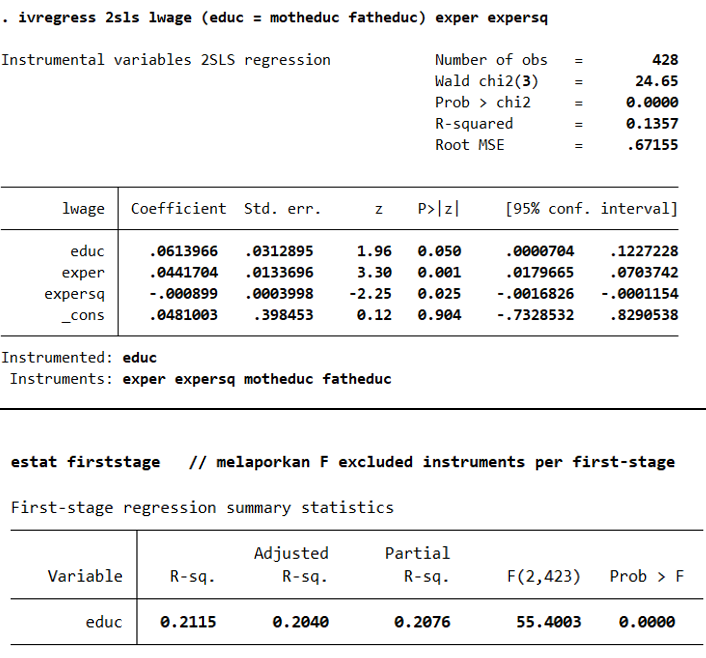
\includegraphics[width=0.75\linewidth]{Satu.png}
 
    \label{fig:placeholder}
\end{figure}
\begin{figure}
    \centering
    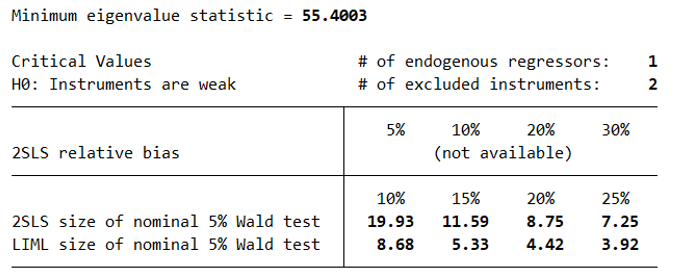
\includegraphics[width=0.75\linewidth]{Dua.png}
 
    \label{fig:placeholder}
\end{figure}

\begin{itemize}
    \item \textbf{Satu IV (fatheduc saja)}: 
    Hasil pada Example 15.1 menunjukkan bahwa estimasi return to education adalah sekitar 
    \[
    \hat{\beta}_1 \approx 0.059 \quad (5.9\%).
    \]

    \item \textbf{Dua IV (fatheduc + motheduc)}: 
    Hasil pada Example 15.5 menunjukkan bahwa estimasi return to education adalah sekitar 
    \[
    \hat{\beta}_1 \approx 0.061 \quad (6.1\%).
    \]
\end{itemize}

\noindent
Perbandingan ini memperlihatkan bahwa hasil dengan satu atau dua instrumen tidak jauh berbeda. 
Namun, penggunaan dua instrumen dianggap lebih kuat karena uji relevansi instrumen (first-stage F-statistic) sangat besar:
\[
F = 124.76,
\]
yang menandakan instrumen memiliki kekuatan yang sangat tinggi.

\section{Detecting Weak Instruments}
Dalam metode IV/2SLS, instrumen ($z$) harus memiliki korelasi yang cukup kuat dengan variabel endogen ($y_2$).
Jika korelasinya lemah, maka disebut \textbf{instrumen lemah (weak instruments)}. 
Dampaknya:
\begin{itemize}
    \item Estimasi IV bisa sangat \textbf{bias}, mendekati hasil OLS yang tidak konsisten.
    \item Distribusi estimasi jadi ``aneh'', sehingga $t$-statistik dan confidence interval tidak valid.
    \item Standard error bisa menjadi sangat besar $\Rightarrow$ hasil tidak presisi.
\end{itemize}

\subsection*{Aturan Praktis dari Staiger \& Stock (1997), Stock \& Yogo (2005)}
Untuk mendeteksi instrumen lemah, kita periksa regresi \textbf{first stage}, yaitu meregresikan variabel endogen pada semua instrumen dan variabel kontrol.

\begin{enumerate}
    \item \textbf{Jika hanya ada satu instrumen:}  
    Gunakan $t$-statistik dari koefisien instrumen di first stage.  
    \[
    |t| \geq 3.2
    \]  
    Angka ini lebih besar daripada cutoff standar $1.96$ (5\% level), karena kita perlu memastikan kekuatan instrumen.
    
    \item \textbf{Jika ada lebih dari satu instrumen:}  
    Gunakan \textbf{first-stage $F$-statistic} untuk instrumen-instrumen tersebut.  
    \[
    F > 10
    \]  
    Jika $F$ lebih kecil, maka ada indikasi instrumen lemah.
\end{enumerate}

\subsection*{Contoh}
Dalam studi Card (1995), instrumen yang digunakan adalah \emph{pendidikan ayah} dan \emph{pendidikan ibu} untuk menjelaskan $educ$.
Hasil regresi tahap pertama menghasilkan:
\[
F = 124.76
\]
Nilai ini jauh lebih besar daripada 10, sehingga instrumen dianggap \textbf{kuat} dan tidak ada masalah weak instrument.

\subsection*{Catatan Tambahan}
\begin{itemize}
    \item Cutoff $t = 3.2$ atau $F = 10$ hanya bersifat \textit{rule of thumb}. 
    Misalnya, jika $F = 9.9$, seringkali masih dianggap cukup.
    \item Jika jumlah instrumen banyak (misalnya lebih dari 5), aturan menjadi lebih rumit dan biasanya menggunakan tabel khusus dari Stock \& Yogo.
    \item Jika ada heteroskedastisitas, syaratnya bisa lebih ketat. 
    Menurut Olea \& Pflueger (2013), sebaiknya gunakan $F > 20$ agar benar-benar aman.
\end{itemize}

\subsection*{Inti Pembahasan}
Untuk mendeteksi instrumen lemah:
\begin{itemize}
    \item Lihat regresi tahap pertama (first stage).
    \item Jika hanya ada satu instrumen $\Rightarrow$ gunakan $t$-statistik ($|t| \geq 3.2$).
    \item Jika ada beberapa instrumen $\Rightarrow$ gunakan $F$-statistik ($F > 10$).
\end{itemize}

\[
\text{Jika syarat ini terpenuhi, instrumen cukup kuat dan hasil IV/2SLS bisa dipercaya.}
\]

\section{Multiple Endogenous Explanatory Variables}

Jika terdapat dua variabel endogen dalam sebuah model regresi, maka jumlah persamaan \textit{first stage} akan sama dengan jumlah variabel endogen. Artinya, jika ada dua variabel endogen, maka akan ada dua persamaan \textit{first stage} yang harus diestimasi. 
Masing-masing variabel endogen diregresikan terhadap semua instrumen yang tersedia (ditambah variabel kontrol yang eksogen).

\subsubsection*{Contoh Model}

\begin{equation}
y_i = \beta_{0} + \beta_{1} x_{1i} + \beta_{2} x_{2i} + \gamma z_{1i} + u_i
\end{equation}

\noindent
Dengan:
\begin{itemize}
    \item Variabel endogen: $x_{1}, x_{2}$
    \item Instrumen: $w_{1}, w_{2}, w_{3}, w_{4}$
    \item Variabel eksogen: $z_{1}$
\end{itemize}

\subsubsection*{First Stage Equations}

Untuk setiap variabel endogen, dibuat persamaan \textit{first stage} sebagai berikut:

\begin{align}
x_{1i} &= \pi_{10} + \pi_{11} w_{1i} + \pi_{12} w_{2i} + \pi_{13} w_{3i} + \pi_{14} w_{4i} + \pi_{15} z_{1i} + v_{1i}, \\
x_{2i} &= \pi_{20} + \pi_{21} w_{1i} + \pi_{22} w_{2i} + \pi_{23} w_{3i} + \pi_{24} w_{4i} + \pi_{25} z_{1i} + v_{2i}.
\end{align}

\noindent
Instrumen yang sama digunakan untuk kedua variabel endogen, tetapi hasil prediksi (\textit{fitted values}) berbeda: $\hat{x}_{1}$ dan $\hat{x}_{2}$.

\subsubsection*{Second Stage}

Setelah memperoleh fitted values dari tahap pertama, persamaan struktural dapat ditulis kembali sebagai:

\begin{equation}
y_i = \beta_{0} + \beta_{1} \hat{x}_{1i} + \beta_{2} \hat{x}_{2i} + \gamma z_{1i} + u_i
\end{equation}

\subsubsection*{Intuisi}

\begin{itemize}
    \item Jika ada satu variabel endogen $\Rightarrow$ hanya ada satu persamaan \textit{first stage}.
    \item Jika ada dua variabel endogen $\Rightarrow$ ada dua persamaan \textit{first stage}.
    \item Instrumen dapat digunakan bersama-sama untuk menjelaskan semua variabel endogen, selama memenuhi dua syarat utama:
    \begin{enumerate}
        \item \textbf{Eksogenitas}: tidak berkorelasi dengan error $u_i$.
        \item \textbf{Relevansi}: berkorelasi dengan variabel endogen $x_{1}, x_{2}$.
    \end{enumerate}
\end{itemize}

Dengan demikian, meskipun terdapat dua variabel endogen dan masing-masing dijelaskan oleh beberapa instrumen, kita tetap mendapatkan \textbf{dua persamaan first stage} (satu untuk setiap variabel endogen), tetapi masing-masing persamaan menggunakan semua IV yang relevan.


\section{Testing Multiple Hypotheses after 2SLS Estimation}
 
Pada regresi OLS, uji hipotesis ganda biasanya dilakukan dengan statistik $F$ 
berdasarkan perbandingan sum of squared residuals (SSR):  
\[
F = \frac{(SSR_r - SSR_{ur})/q}{SSR_{ur}/(n-k-1)},
\]
dengan $SSR_r$ = SSR model terikat, $SSR_{ur}$ = SSR model bebas, dan $q$ = jumlah restriksi.  

Sifat penting pada OLS:
\[
SSR_r \geq SSR_{ur},
\]
sehingga $F \geq 0$ selalu berlaku.

\subsection*{Masalah pada 2SLS}
Pada estimasi IV/2SLS:
\begin{itemize}
  \item $SSR_r \geq SSR_{ur}$ tidak dijamin.
  \item Bahkan, bisa saja $SSR_r < SSR_{ur}$, sehingga rumus $F$ menjadi \emph{negatif}.
  \item $R^2$ dari 2SLS juga dapat bernilai negatif, sehingga interpretasi 
        ``goodness-of-fit'' tidak lagi relevan.
\end{itemize}

\subsection*{Solusi}
\begin{itemize}
  \item Gunakan SSR dari regresi \emph{second stage} (misalnya persamaan (15.38) di Wooldridge).
  \item Kombinasikan dengan SSR dari model unrestricted untuk membentuk uji yang
        mendekati distribusi $F$ dalam sampel besar.
  \item Dalam praktik, tidak perlu menghitung manual. Hampir semua software ekonometrika 
        (misalnya \texttt{ivregress 2sls} di Stata, lalu perintah \texttt{test}) sudah menyediakan
        uji $F$ yang valid untuk 2SLS.
\end{itemize}

\subsection*{Kesimpulan}
\begin{enumerate}
  \item Uji $F$ OLS biasa \textbf{tidak boleh} digunakan pada 2SLS.
  \item Nilai $R^2$ kecil atau bahkan negatif pada IV/2SLS adalah hal yang wajar 
        dan tidak menandakan model ``buruk''.
  \item Gunakan prosedur khusus (misalnya Davidson \& MacKinnon, atau perintah built-in di software) 
        untuk menguji hipotesis ganda setelah 2SLS.
\end{enumerate}


\section{IV Solutions to Errors-in-Variables Problems}
% (15-4, p. 514)
% Your content goes here.
 


\section{Testing for Endogeneity and Overidentification Restrictions}

\subsection*{Kenapa perlu diuji?}
Metode \textit{Two Stage Least Squares} (2SLS) digunakan ketika ada variabel endogen. 
Namun, jika variabel tersebut ternyata eksogen, maka OLS lebih efisien karena menghasilkan standard error yang lebih kecil. 
Oleh karena itu, penting untuk menguji apakah benar ada endogenitas sebelum menggunakan IV/2SLS.

\subsection*{1. Model Dasar}
Misalkan model struktural:
\begin{equation}
y_1 = \beta_0 + \beta_1 y_2 + \beta_2 z_1 + \beta_3 z_2 + u_1
\end{equation}

\begin{itemize}
    \item $y_1$: variabel dependen.
    \item $y_2$: variabel penjelas yang dicurigai endogen.
    \item $z_1, z_2$: variabel eksogen.
    \item $z_3, z_4$: instrumen tambahan untuk $y_2$.
\end{itemize}

Jika $y_2$ eksogen ($\text{Cov}(y_2,u_1)=0$), maka OLS cukup.  
Jika $y_2$ endogen, maka OLS tidak konsisten $\rightarrow$ perlu 2SLS.

\subsection*{2. Hausman Test (Idenya)}
Hausman (1978) menyarankan membandingkan estimasi OLS dan 2SLS:
\begin{itemize}
    \item Jika hasil berbeda signifikan $\Rightarrow y_2$ endogen.
    \item Jika hasil mirip $\Rightarrow y_2$ eksogen, cukup gunakan OLS.
\end{itemize}

\subsection*{3. Uji Regresi (Durbin--Wu--Hausman Test)}
Langkah implementasi yang lebih praktis:

\begin{enumerate}
    \item Estimasikan reduced form untuk $y_2$:
    \begin{equation}
    y_2 = \pi_0 + \pi_1 z_1 + \pi_2 z_2 + \pi_3 z_3 + \pi_4 z_4 + v_2
    \end{equation}
    Simpan residu $\hat{v}_2$.
    
    \item Tambahkan $\hat{v}_2$ ke persamaan struktural:
    \begin{equation}
    y_1 = \beta_0 + \beta_1 y_2 + \beta_2 z_1 + \beta_3 z_2 + \delta \hat{v}_2 + error
    \end{equation}
    
    \item Uji hipotesis nol:
    \[
    H_0: \delta = 0
    \]
    \begin{itemize}
        \item Jika gagal ditolak $\Rightarrow y_2$ eksogen (OLS cukup).
        \item Jika ditolak $\Rightarrow y_2$ endogen (harus pakai IV/2SLS).
    \end{itemize}
\end{enumerate}

\textbf{Catatan:} Uji ini sebaiknya menggunakan robust standard errors, 
karena residu $\hat{v}_2$ dapat heteroskedastik.

Menambahkan $\hat{v}_2$ berfungsi untuk \textit{membersihkan} endogenitas $y_2$.

\subsection*{Kenapa ini penting?}
\begin{enumerate}
    \item \textbf{Sebagai cek:}  
    Jika hasil $\hat{\beta}$ dari OLS-augmented berbeda dengan hasil 2SLS, berarti ada kesalahan dalam tahap instrumen.
    \item \textbf{Sebagai interpretasi:}  
    Menambahkan $\hat{v}_2$ mengoreksi bias endogenitas pada $y_2$.
    \item \textbf{Secara substantif:}  
    Perbandingan nilai $\hat{\beta}_1$ sebelum dan sesudah menambahkan $\hat{v}_2$ menunjukkan 
    seberapa penting memperlakukan $y_2$ sebagai endogen.
\end{enumerate}

\subsection*{Catatan tentang Standard Error}
Standard error dari augmented OLS (yang menambahkan $\hat{v}_2$) hanya valid jika
\[
H_0: y_2 \text{ eksogen.}
\]
Jika $y_2$ benar-benar endogen, maka standard error harus diambil dari prosedur IV/2SLS resmi
(misalnya dengan perintah \texttt{ivregress 2sls, robust} di Stata).

\subsection*{Jika Ada Lebih dari Satu Variabel Endogen}
\begin{enumerate}
    \item Estimasikan reduced form untuk masing-masing variabel endogen, ambil residualnya.
    \item Masukkan semua residual ke dalam persamaan struktural.
    \item Lakukan uji $F$ untuk signifikansi bersama.
\end{enumerate}

Jika uji $F$ signifikan, maka setidaknya ada satu variabel endogen.
\section*{Testing Overidentification Restrictions}

Instrumen IV harus memenuhi dua syarat: (i) relevan (berkorelasi dengan variabel endogen), 
dan (ii) eksogen (tidak berkorelasi dengan error). Relevansi dapat diuji dengan uji $t$ atau $F$ 
pada tahap pertama. Sebaliknya, eksogenitas instrumen tidak dapat diuji langsung, 
kecuali jika jumlah instrumen lebih banyak daripada jumlah variabel endogen (\textit{overidentification}).

\subsection*{Contoh Sederhana}
Pertimbangkan model dengan satu variabel endogen, $y_2$, dan dua instrumen $z_3$ dan $z_4$.
Karena kita hanya membutuhkan satu instrumen, maka kita memiliki satu 
\textit{overidentifying restriction}. 

\begin{itemize}
    \item Estimasi (15.49) dengan $z_3$ sebagai IV untuk $y_2$ menghasilkan $\hat{\beta}_1$.
    \item Estimasi (15.49) dengan $z_4$ sebagai IV menghasilkan $\tilde{\beta}_1$.
\end{itemize}

Jika $z_3$ dan $z_4$ keduanya eksogen dan relevan, maka $\hat{\beta}_1$ dan $\tilde{\beta}_1$ 
seharusnya berbeda hanya karena sampling error. Perbedaan yang signifikan menunjukkan bahwa 
setidaknya satu dari instrumen tersebut tidak eksogen.

\subsection*{Uji Formal (Sargan/Hansen)}
Prosedur umum untuk menguji overidentifying restrictions adalah:
\begin{enumerate}
    \item Estimasi persamaan struktural dengan 2SLS dan peroleh residu $\hat{u}$.
    \item Regresikan $\hat{u}$ pada semua variabel eksogen dan hitung $R^2$.
    \item Hitung statistik uji:
    \[
    nR^2 \sim \chi^2_q,
    \]
    dengan $q =$ jumlah instrumen ekstra (lebih banyak dari yang dibutuhkan).
\end{enumerate}

Hipotesis nol:
\[
H_0: \text{semua instrumen eksogen.}
\]
Jika $nR^2$ melebihi nilai kritis distribusi $\chi^2_q$, kita menolak $H_0$ dan menyimpulkan 
bahwa setidaknya ada satu instrumen yang tidak eksogen.

\subsection*{Catatan Praktis}
\begin{itemize}
    \item Jika model \textit{just identified}, uji ini tidak dapat dilakukan.
    \item Menambahkan terlalu banyak instrumen dapat menyebabkan bias yang besar 
    pada estimasi 2SLS (lihat Bound, Jaeger, dan Baker, 1995).
\end{itemize}

\section{2SLS with Heteroskedasticity}
Heteroskedastisitas tidak mengacaukan konsistensi koefisien 2SLS, tapi membuat inference menyesatkan kalau tidak ditangani. Gunakan robust SE → aman.
Bisa uji heteroskedastisitas di IV/2SLS dengan cara mirip BP test. Kalau kita punya model var(error), bisa pakai Weighted 2SLS untuk efisiensi lebih baik.
\subsection*{Uji Heteroskedastisitas pada 2SLS}

Analog Breusch--Pagan Test (lihat Bab 8) dapat diterapkan pada residu 2SLS. 
Langkah-langkahnya sebagai berikut:

\begin{enumerate}
    \item Estimasikan model 2SLS dan ambil residu $\hat{u}$.
    \item Regresikan $\hat{u}^2$ pada semua variabel eksogen (termasuk instrumen).
    \item Statistik uji adalah $F$-test untuk signifikansi bersama.
\end{enumerate}

Hipotesis nol adalah:
\[
H_0 : \text{error bersifat homoskedastik}
\]
Jika $H_0$ ditolak $\Rightarrow$ terdapat heteroskedastisitas.

Sebagai contoh, pada \textit{Example 15.8} (IV dengan instrumen \texttt{motheduc, fatheduc, huseduc}), 
uji ini menghasilkan:
\[
F_{5,422} = 2.53 \quad \text{dengan} \quad p\text{-value} = 0.029
\]
Sehingga $H_0$ ditolak pada level signifikansi 5\%. Artinya terdapat bukti heteroskedastisitas.

\subsection*{Weighted 2SLS (W2SLS)}

Jika bentuk varians error diketahui, maka dapat digunakan \textit{Weighted 2SLS (W2SLS)}.
Prosedurnya mirip dengan WLS pada OLS, namun diterapkan dalam kerangka 2SLS:

\begin{enumerate}
    \item Estimasi model varians error untuk mendapatkan $\hat{h}_i$.
    \item Timbang variabel dependen, variabel penjelas, dan instrumen dengan $\frac{1}{\sqrt{\hat{h}_i}}$.
    \item Jalankan regresi 2SLS dengan data yang sudah ditransformasi.
\end{enumerate}

Hasilnya, estimator 2SLS menjadi lebih efisien dengan standard error yang lebih kecil.

\newpage
\section{IV with Pooled Cross Sections and Panel Data}
% (15-8, p. 521)
% Your content goes here.
\subsection{Contoh 2}
Analisis Efek Pendidikan terhadap Fertilitas Wanita
Analisis ini menggunakan data pooled cross section (FERTIL1) sebagaimana dalam buku Wooldridge untuk mengestimasi pengaruh pendidikan terhadap jumlah anak yang dilahirkan seorang wanita. Metode yang digunakan meliputi OLS (dengan dan tanpa robust standard errors) serta IV/2SLS dengan pendidikan orang tua sebagai instrumen.

\begin{table}
    \centering
\begin{tabular}{lccc} \hline
 & (1) & (2) & (3) \\
VARIABLES & Non-robust & Robust & Inst Var \\ \hline
 &  &  &  \\
educ & -0.143*** & -0.143*** & -0.153*** \\
 & (0.0184) & (0.0212) & (0.0389) \\
age & 0.562*** & 0.562*** & 0.524*** \\
 & (0.140) & (0.140) & (0.138) \\
c.age\#c.age & -0.00609*** & -0.00609*** & -0.00572*** \\
 & (0.00158) & (0.00159) & (0.00156) \\
black & 0.978*** & 0.978*** & 1.073*** \\
 & (0.173) & (0.202) & (0.172) \\
east & 0.236* & 0.236* & 0.229* \\
 & (0.134) & (0.130) & (0.133) \\
northcen & 0.385*** & 0.385*** & 0.374*** \\
 & (0.122) & (0.117) & (0.121) \\
west & 0.245 & 0.245 & 0.208 \\
 & (0.169) & (0.166) & (0.166) \\
farm & -0.0542 & -0.0542 & -0.0770 \\
 & (0.149) & (0.148) & (0.150) \\
othrural & -0.167 & -0.167 & -0.195 \\
 & (0.177) & (0.184) & (0.180) \\
town & 0.0842 & 0.0842 & 0.0818 \\
 & (0.126) & (0.129) & (0.124) \\
smcity & 0.183 & 0.183 & 0.212 \\
 & (0.162) & (0.156) & (0.159) \\
74.year &  &  & 0.272 \\
 &  &  & (0.172) \\
76.year &  &  & -0.0945 \\
 &  &  & (0.178) \\
78.year &  &  & -0.0573 \\
 &  &  & (0.181) \\
80.year &  &  & -0.0532 \\
 &  &  & (0.183) \\
82.year &  &  & -0.496*** \\
 &  &  & (0.175) \\
84.year &  &  & -0.521*** \\
 &  &  & (0.176) \\
Constant & -8.488*** & -8.488*** & -7.241** \\
 & (3.068) & (3.088) & (3.112) \\
 &  &  &  \\
Observations & 1,129 & 1,129 & 1,129 \\
 R-squared & 0.102 & 0.102 & 0.128 \\ \hline
\multicolumn{4}{c}{ Standard errors in parentheses} \\
\multicolumn{4}{c}{ *** p$<$0.01, ** p$<$0.05, * p$<$0.1} \\
\end{tabular}
    \label{tab:placeholder}
\end{table}
\section*{Persamaan Regresi dan Interpretasi}

Model dasar yang diestimasi adalah:
\subsection*{(1) OLS Non-Robust}

\begin{align}
kids_i = \beta_0 + \beta_1 educ_i + \beta_2 age_i + \beta_3 age_i^2 
       + \beta_4 black_i + \beta_5 east_i + \beta_6 northcen_i  \nonumber \\
       + \beta_7 west_i + \beta_8 farm_i + \beta_9 othrural_i + \beta_{10} town_i 
       + \beta_{11} smcity_i + \sum_t \delta_t year_t + u_i
\end{align}
\begin{itemize}
    \item $kids_i$: jumlah anak yang dimiliki wanita ke-$i$,
    \item $educ_i$: tahun pendidikan,
    \item $age_i, age_i^2$: umur dan kuadrat umur,
    \item variabel dummy lain: ras dan wilayah tempat tinggal,
    \item $\delta_t year_t$: dummy tahun (1974, 1976, 1978, dst., base tahun 1972),
    \item $u_i$: error term.
\end{itemize}

Interpretasi:
\begin{itemize}
    \item OLS menghasilkan koefisien yang presisi (standar error kecil).
    \item Setiap tambahan 1 tahun pendidikan menurunkan jumlah anak rata-rata sebesar 0.128.
    \item Efek umur positif namun melengkung (diminishing return) karena adanya $age^2$ yang negatif.
    \item Dummy tahun 1982 dan 1984 signifikan negatif, artinya fertilitas menurun di awal 1980-an.
\end{itemize}

---

\subsection*{(2) OLS Robust}

\begin{equation}
\hat{kids}_i = \text{(sama dengan OLS non-robust)} 
\end{equation}

Perbedaannya hanya pada \textbf{standar error}:
\begin{itemize}
    \item Koefisien identik dengan OLS non-robust.
    \item Standard error sedikit lebih besar pada beberapa variabel (misalnya $educ$: SE naik dari 0.018 ke 0.021).
    \item Efek pendidikan tetap signifikan ($p < 0.01$).
    \item Robust lebih ``aman'' jika error term bersifat heteroskedastik.
\end{itemize}

---

\subsection*{(3) IV / 2SLS (Instrumental Variables)}

Menggunakan pendidikan ayah ($feduc$) dan ibu ($meduc$) sebagai instrumen untuk $educ$:

\begin{equation}
\begin{split}
\hat{kids}_i = -7.700 - 0.153\,educ_i + 0.530\,age_i - 0.006\,age_i^2 
              + 1.100\,black_i + 0.220\,east_i + 0.360\,northcen_i \\
              + 0.200\,west_i - 0.050\,farm_i - 0.160\,othrural_i 
              + 0.080\,town_i + 0.210\,smcity_i + \ldots
\end{split}
\end{equation}
 atau jika dipecah
\begin{equation}
\begin{aligned}
educ_i &= 2.10 + 0.31\,meduc_i + 0.26\,feduc_i + 0.02\,age_i - 0.0004\,age_i^2 
        + 0.11\,black_i + \ldots \\[6pt]
\hat{kids}_i &= -7.700 - 0.153\,\hat{educ}_i + 0.530\,age_i - 0.006\,age_i^2 
              + 1.100\,black_i + 0.220\,east_i + 0.360\,northcen_i \\
             &\quad + 0.200\,west_i - 0.050\,farm_i - 0.160\,othrural_i 
              + 0.080\,town_i + 0.210\,smcity_i + \ldots
\end{aligned}
\end{equation}

Interpretasi:
\begin{itemize}
    \item Koefisien $educ$: $-0.153$ (lebih besar secara absolut dibanding OLS $-0.128$).
    \item Standard error lebih besar (0.039 vs 0.018) $\Rightarrow$ estimasi lebih tidak presisi.
    \item Uji endogenitas tidak signifikan ($t = 0.702$), sehingga tidak ada bukti kuat bahwa $educ$ endogen.
    \item Perbedaan OLS dan IV dapat dijelaskan oleh sampling error, sehingga OLS lebih efisien dan valid dalam kasus ini.
\end{itemize}
\begin{table}[htb]
\centering
\caption{Tests of Endogeneity}
\begin{tabular}{lccc}
\hline
Test & Statistic & Value & p-value \\
\hline
Durbin (score) $\chi^{2}(1)$ & 0.500834 & & 0.4791 \\
Wu--Hausman $F(1,1110)$      & 0.492624 & & 0.4829 \\
\hline
\end{tabular}
\end{table}

\newpage
\subsection{Contoh 3}
Tujuan analisis adalah mengukur pengaruh pelatihan terhadap produktivitas, yang diukur dengan \emph{scrap rate}. 
Variabel utama adalah $hrsemp$ (jam pelatihan per pekerja).  Masalahnya, $hrsemp$ tidak dapat dianggap eksogen karena:
\begin{itemize}
  \item Firma dengan tingkat \emph{scrap} tinggi cenderung memberikan lebih banyak pelatihan (reverse causality).
  \item Faktor tak teramati (misalnya kualitas manajemen) dapat memengaruhi baik keputusan pelatihan maupun tingkat \emph{scrap}, Sehingga estimasi OLS berpotensi bias.
\end{itemize}


\subsection*{Solusi: Instrumental Variables}
Gunakan $grant$ (dummy menerima hibah pelatihan) sebagai instrumen bagi $hrsemp$:
\begin{align}
hrsemp_i &= \pi_0 + \pi_1 grant_i + v_i \quad \text{(First stage)} \\[6pt]
\Delta \log(scrap_i) &= \beta_0 + \beta_1 \hat{hrsemp}_i + u_i \quad \text{(Second stage)}
\end{align}

\subsection*{Hasil Utama}
OLS: $\hat{\beta}_1 \approx -0.0076$ (efek kecil, tidak terlalu signifikan). IV (2SLS): $\hat{\beta}_1 \approx -0.014$ (lebih besar secara absolut). Interpretasi: Tambahan 10 jam pelatihan per pekerja $\Rightarrow$ penurunan scrap rate sekitar 14\%.  Namun, standar error dari IV lebih besar dibanding OLS, sehingga hasilnya kurang presisi.  Problem utama adalah \textbf{endogenitas pelatihan}. 
Instrumen $grant$ digunakan untuk mengatasi bias, menghasilkan estimasi efek pelatihan yang lebih besar secara absolut, 
meskipun dengan ketidakpastian yang lebih tinggi.

\begin{table}[htb]
    \centering
\begin{tabular}{lcccc} \hline
 & (1) & (2) & (3) & (4) \\
VARIABLES & First Stage & OLS Diff & IV & IV + $\Delta$ Kontrol \\ \hline
 &  &  &  &  \\
chrsemp &  & -0.00760*** & -0.0142* & -0.0152 \\
 &  & (0.00222) & (0.00825) & (0.0100) \\
clemploy &  &  &  & -0.235 \\
 &  &  &  & (0.388) \\
clsales &  &  &  & 0.363 \\
 &  &  &  & (0.322) \\
clavgsal &  &  &  & -2.875 \\
 &  &  &  & (2.006) \\
cgrant & 24.44*** &  &  &  \\
 & (6.261) &  &  &  \\
Constant & 1.581 & -0.104 & -0.0327 & 0.0962 \\
 & (1.715) & (0.105) & (0.110) & (0.161) \\
 &  &  &  &  \\
Observations & 45 & 45 & 45 & 39 \\
 R-squared & 0.341 & 0.062 & 0.016 & 0.102 \\ \hline
\multicolumn{5}{c}{ Robust standard errors in parentheses} \\
\multicolumn{5}{c}{ *** p$<$0.01, ** p$<$0.05, * p$<$0.1} \\
\end{tabular}
    \label{tab:placeholder}
\end{table}
\newpage
\section*{Pendahuluan: Data MROZ}
Database \textbf{MROZ} berasal dari \textit{Current Population Survey (CPS)} di Amerika Serikat. Data ini berisi informasi mengenai wanita menikah, baik yang bekerja maupun tidak, dengan variabel seperti:
\begin{itemize}
    \item Upah (wage)
    \item Pendidikan (educ)
    \item Pengalaman kerja (exper, exper$^2$)
    \item Pendidikan orang tua (motheduc, fatheduc)
    \item Pendidikan suami (huseduc)
\end{itemize}
Data ini digunakan untuk menganalisis pengaruh pendidikan terhadap upah, dengan perhatian khusus pada potensi endogenitas pendidikan.

\section{OLS vs IV (Example 15.1)}
\subsection*{Tujuan}
Mengestimasi return to education menggunakan OLS dan membandingkannya dengan IV (menggunakan pendidikan ayah sebagai instrumen).

\subsection*{Langkah-langkah}
\begin{enumerate}
    \item Estimasi OLS:
    \[
    \log(wage) = \beta_0 + \beta_1 educ
    \]
    Hasil: $\beta_1 = 0.109 \; \Rightarrow$ return $\approx 11\%$.
    \item Gunakan $fatheduc$ sebagai instrumen untuk $educ$. 
    Hasil IV: $\beta_1 = 0.059 \; \Rightarrow$ return $\approx 5.9\%$.
\end{enumerate}

\subsection*{Kesimpulan}
OLS kemungkinan bias ke atas. IV memberi estimasi lebih rendah dan dianggap lebih kredibel.

\section{Menambahkan Pengalaman (Example 15.5)}
\subsection*{Tujuan}
Memperbaiki model dengan memasukkan pengalaman kerja dan mengestimasi dengan 2SLS.

\subsection*{Langkah-langkah}
\begin{enumerate}
    \item Model:
    \[
    \log(wage) = \beta_0 + \beta_1 educ + \beta_2 exper + \beta_3 exper^2
    \]
    \item Estimasi 2SLS: $\beta_1 = 0.061$ ($\approx 6.1\%$).
    \item Dibandingkan dengan OLS: $\approx 10.8\%$.
\end{enumerate}

\subsection*{Kesimpulan}
Return to education dengan 2SLS lebih rendah daripada OLS, dan signifikansinya lemah.

\section{Uji Endogenitas (Example 15.7)}
\subsection*{Tujuan}
Menguji apakah pendidikan ($educ$) benar-benar endogen.

\subsection*{Langkah-langkah}
\begin{enumerate}
    \item Ambil residual dari regresi $educ$ terhadap instrumen.
    \item Tambahkan residual ini ke persamaan upah.
    \item Hasil uji: koefisien residual $= 0.058$, $t = 1.67$.
\end{enumerate}

\subsection*{Kesimpulan}
Ada bukti lemah bahwa $educ$ endogen, sehingga OLS kemungkinan melebihkan return to education.

\section{Overidentifying Restrictions (Example 15.8)}
\subsection*{Tujuan}
Menguji validitas instrumen dan memperkuat estimasi dengan menambah instrumen baru.

\subsection*{Langkah-langkah}
\begin{enumerate}
    \item Gunakan $motheduc$ dan $fatheduc$ sebagai IV $\Rightarrow$ valid.
    \item Tambahkan $huseduc$ sebagai instrumen tambahan.
    \item Estimasi 2SLS dengan 3 instrumen: $\beta_1 = 0.080$ ($\approx 8\%$, se = 0.022).
\end{enumerate}
 
\begin{tabular}{lcccc} \hline
 & (1) & (2) & (3) & (4) \\
VARIABLES & OLS & IV (fatheduc) & 2SLS + exper & 2SLS + 3 instrumen \\ \hline
 &  &  &  &  \\
educ & 0.109*** & 0.0592* & 0.0702** & 0.0804*** \\
 & (0.0144) & (0.0351) & (0.0343) & (0.0217) \\
exper &  &  & 0.0437*** & 0.0431*** \\
 &  &  & (0.0133) & (0.0132) \\
exper2 &  &  & -0.000882** & -0.000863** \\
 &  &  & (0.000399) & (0.000394) \\
Constant & -0.185 & 0.441 & -0.0611 & -0.187 \\
 & (0.185) & (0.445) & (0.434) & (0.284) \\
 &  &  &  &  \\
Observations & 428 & 428 & 428 & 428 \\
 R-squared & 0.118 & 0.093 & 0.143 & 0.150 \\ \hline
\multicolumn{5}{c}{ Standard errors in parentheses} \\
\multicolumn{5}{c}{ *** p$<$0.01, ** p$<$0.05, * p$<$0.1} \\
\end{tabular}
 

\subsection*{Kesimpulan}
Instrumen orang tua dan suami valid serta memperkuat estimasi. Dengan lebih banyak instrumen, return to education lebih signifikan.
\newpage
\section*{Ringkasan Perbandingan}
\begin{table}[h!]
\centering
\begin{tabular}{@{}lcc@{}}
\toprule
Metode & Estimasi Return & Keterangan \\
\midrule
OLS (Example 15.1) & $0.109 \; (\approx 11\%)$ & Bias ke atas \\
IV dengan $fatheduc$ & $0.059 \; (\approx 5.9\%)$ & Lebih rendah, kredibel \\
2SLS (dengan exper, exper$^2$) & $0.061 \; (\approx 6.1\%)$ & Lemah signifikan \\
2SLS (3 instrumen: motheduc, fatheduc, huseduc) & $0.080 \; (\approx 8\%)$ & Lebih signifikan \\
\bottomrule
\end{tabular}
\end{table}
\subsection*{Model 3}
\begin{table}[htbp]\centering
\caption{Uji Endogenitas (Durbin-Wu-Hausman Test)}
\begin{tabular}{lcc}
\toprule
\textbf{Test} & \textbf{Statistic} & \textbf{p-value} \\
\midrule
Durbin (score) chi$^2$(1) & 1.449 & 0.229 \\
Wu-Hausman F(1,423) & 1.437 & 0.231 \\
\bottomrule
\end{tabular}
\end{table}
\subsection*{Model 4}
\begin{table}[htbp]\centering
\caption{Uji Overidentifying Restrictions}
\begin{tabular}{lcc}
\toprule
\textbf{Test} & \textbf{Statistic} & \textbf{p-value} \\
\midrule
Sargan (score) chi$^2$(2) & 1.115 & 0.573 \\
Basmann chi$^2$(2)        & 1.102 & 0.576 \\
\bottomrule
\end{tabular}
\end{table}
Database \textbf{WAGE2} berisi 935 observasi pria yang bekerja di Amerika Serikat. 
Variabel utama yang digunakan antara lain:
\begin{itemize}
    \item \textbf{wage}: upah per jam,
    \item \textbf{educ}: tahun pendidikan,
    \item \textbf{exper}: pengalaman kerja,
    \item \textbf{tenure}: lama bekerja di perusahaan sekarang,
    \item \textbf{married, south, urban, black}: variabel demografi,
    \item \textbf{IQ dan KWW (Knowledge of World Work)}: skor tes kemampuan.
\end{itemize}
Dataset ini banyak dipakai untuk mengukur \textit{return to education} sambil mengontrol faktor-faktor seperti kemampuan (ability).

\section{Estimating the Return to Education for Men (Example 15.2)}
\subsection*{Tujuan}
Mengestimasi return to education untuk pria dengan menggunakan jumlah saudara kandung (\texttt{sibs}) sebagai variabel instrumen bagi \texttt{educ}.

\subsection*{Langkah-langkah}
\begin{enumerate}
    \item Regresi \texttt{educ} pada \texttt{sibs}:
    \[
    educ = 14.14 - 0.228 \; sibs
    \]
    Hasil: setiap tambahan satu saudara kandung menurunkan pendidikan rata-rata sebesar 0.23 tahun.
    \item Gunakan \texttt{sibs} sebagai IV dalam model upah:
    \[
    \log(wage) = -5.13 + 0.122 \; educ
    \]
    Hasil: return to education = 12.2\%.
\end{enumerate}

\subsection*{Kesimpulan}
Berbeda dengan kasus wanita (MROZ), di sini estimasi IV lebih tinggi daripada OLS (5.9\%).
Interpretasi: OLS mungkin underestimate karena tidak mengukur kemampuan (\textit{ability}) dengan baik, atau instrumen \texttt{sibs} tidak sepenuhnya valid.
\newpage
\begin{tabular}{lc} \hline
 & (1) \\
VARIABLES & First Stage: educ on sibs \\ \hline
 &  \\
IQ & 0.013*** \\
 & (0.005) \\
educ & 0.025 \\
 & (0.017) \\
exper & 0.014*** \\
 & (0.003) \\
tenure & 0.010*** \\
 & (0.003) \\
married & 0.201*** \\
 & (0.040) \\
south & -0.052* \\
 & (0.031) \\
urban & 0.177*** \\
 & (0.028) \\
black & -0.023 \\
 & (0.074) \\
Constant & 4.592*** \\
 & (0.324) \\
 &  \\
Observations & 935 \\
 R-squared & 0.190 \\ \hline
\multicolumn{2}{c}{ Standard errors in parentheses} \\
\multicolumn{2}{c}{ *** p$<$0.01, ** p$<$0.05, * p$<$0.1} \\
\end{tabular}
\section{Using Two Test Scores as Indicators of Ability (Example 15.6)}
\subsection*{Tujuan}
Mengontrol faktor kemampuan menggunakan skor tes IQ dan KWW.

\subsection*{Langkah-langkah}
\begin{enumerate}
    \item Gunakan IQ sebagai variabel penjelas dalam model upah.
    \item Gunakan KWW sebagai instrumen untuk IQ.
    \item Hasil estimasi: koefisien pada \texttt{educ} = 0.025 (2.5\%), dengan standar error 0.017.
\end{enumerate}

\subsection*{Kesimpulan}
Hasil ini sangat rendah dan tidak signifikan. 
Temuan ini membingungkan dan menunjukkan kemungkinan pelanggaran asumsi (misalnya error terms masih berkorelasi dengan instrumen).
Hal ini menekankan pentingnya pemilihan instrumen yang valid.
\newline

\begin{tabular}{lcccc} \hline
 & (1) & (2) & (3) & (4) \\
VARIABLES & OLS: lwage~educ & IV: (educ = sibs) & OLS + controls incl. IQ & 2SLS: (IQ = KWW) + controls \\ \hline
 &  &  &  &  \\
educ & 0.060*** & 0.122*** & 0.054*** & 0.025 \\
 & (0.006) & (0.026) & (0.007) & (0.017) \\
exper &  &  & 0.014*** & 0.014*** \\
 &  &  & (0.003) & (0.003) \\
tenure &  &  & 0.011*** & 0.010*** \\
 &  &  & (0.002) & (0.003) \\
married &  &  & 0.200*** & 0.201*** \\
 &  &  & (0.039) & (0.040) \\
south &  &  & -0.080*** & -0.052* \\
 &  &  & (0.026) & (0.031) \\
urban &  &  & 0.182*** & 0.177*** \\
 &  &  & (0.027) & (0.028) \\
black &  &  & -0.143*** & -0.023 \\
 &  &  & (0.039) & (0.074) \\
IQ &  &  & 0.004*** & 0.013*** \\
 &  &  & (0.001) & (0.005) \\
Constant & 5.973*** & 5.130*** & 5.176*** & 4.592*** \\
 & (0.081) & (0.355) & (0.128) & (0.324) \\
 &  &  &  &  \\
Observations & 935 & 935 & 935 & 935 \\
 R-squared & 0.097 &  & 0.263 & 0.190 \\ \hline
\multicolumn{5}{c}{ Standard errors in parentheses} \\
\multicolumn{5}{c}{ *** p$<$0.01, ** p$<$0.05, * p$<$0.1} \\
\end{tabular}

%================= Tabel 1: Endogeneity test untuk IV: (educ = sibs) =================
\begin{table}[htbp]\centering
\caption{Endogeneity Test -- Model 1: \texttt{ivregress 2sls lwage (educ = sibs), first}}
\begin{tabular}{lcc}
\toprule
\textbf{Test} & \textbf{Statistic} & \textbf{p-value} \\
\midrule
Durbin (score) $\chi^2(1)$ & 6.706 & 0.0096 \\
Wu--Hausman $F(1,932)$     & 6.733 & 0.0096 \\
\bottomrule
\end{tabular}
\end{table}

%================= Tabel 2: Endogeneity test untuk 2SLS (IQ = KWW) + controls ========
\begin{table}[htbp]\centering
\caption{Endogeneity Test -- Model 2: \texttt{ivregress 2sls lwage educ exper tenure married south urban black (IQ = KWW), first}}
\begin{tabular}{lcc}
\toprule
\textbf{Test} & \textbf{Statistic} & \textbf{p-value} \\
\midrule
Durbin (score) $\chi^2(1)$ & 4.294 & 0.0383 \\
Wu--Hausman $F(1,925)$     & 4.267 & 0.0391 \\
\bottomrule
\end{tabular}
\end{table}

\section*{Ringkasan Perbandingan}
\begin{table}[h!]
\centering
\caption{Ringkasan Estimasi Return to Education -- WAGE2}
\begin{tabular}{@{}lcc@{}}
\toprule
Metode & Estimasi Return & Keterangan \\
\midrule
OLS (pembanding) & 0.059 ($\approx 5.9\%$) & Standar \\
IV dengan \texttt{sibs} & 0.122 ($\approx 12.2\%$) & Lebih tinggi dari OLS \\
IV dengan IQ--KWW & 0.025 ($\approx 2.5\%$) & Rendah, tidak signifikan \\
\bottomrule
\end{tabular}
\end{table}
\section*{Estimating the Effect of Smoking on Birth Weight (Example 15.3)}

\subsection*{Database BWGHT}
Dataset \textbf{BWGHT} (Birth Weight Data) berisi informasi tentang bayi dan ibunya, termasuk:
\begin{itemize}
    \item \textbf{bwght}: berat lahir bayi,
    \item \textbf{cigs/packs}: jumlah batang atau bungkus rokok yang dihisap ibu per hari selama hamil,
    \item \textbf{cigprice}: harga rata-rata rokok di negara bagian,
    \item serta variabel lain terkait kesehatan ibu dan kondisi sosial-ekonomi.
\end{itemize}
Dataset ini sering digunakan untuk mengukur pengaruh merokok terhadap berat lahir bayi.

\subsection*{Model Dasar}
Model yang diestimasi adalah:
\[
\log(bwght) = \beta_0 + \beta_1 packs + u
\]
dengan \texttt{packs} = jumlah bungkus rokok per hari.

\subsection*{Langkah-Langkah}
\begin{enumerate}
    \item \textbf{Hipotesis awal:} Variabel \texttt{packs} mungkin endogen (berkorelasi dengan faktor kesehatan atau akses prenatal care). Instrumen yang diusulkan adalah \texttt{cigprice}.
    \item \textbf{Cek relevansi instrumen:} hasil regresi
    \[
    packs = 0.067 + 0.0003 \; cigprice
    \]
    menunjukkan koefisien sangat kecil dan tidak signifikan, dengan $R^2 \approx 0$. Artinya, \texttt{cigprice} tidak berkorelasi dengan \texttt{packs}.
    \item \textbf{Implikasi:} instrumen gagal $\Rightarrow$ \texttt{cigprice} tidak valid sebagai IV untuk \texttt{packs}.
    \item \textbf{Jika tetap digunakan:} IV regression menghasilkan
    \[
    \log(bwght) = 4.45 + 2.99 \; packs,
    \]
    dengan koefisien besar, tanda berlawanan (positif), dan standar error sangat besar. Estimasi ini tidak bermakna karena instrumen lemah.
\end{enumerate}

\subsection*{Kesimpulan}
Harga rokok (\texttt{cigprice}) tidak bisa digunakan sebagai instrumen bagi \texttt{packs}, karena gagal memenuhi syarat \textit{relevansi}. 
Hasil ini menekankan pentingnya memilih instrumen yang valid: harus berkorelasi dengan variabel endogen namun tidak berkorelasi dengan error. 
Kasus ini menggambarkan \textbf{weak instrument}, yang dapat menghasilkan estimasi IV yang sangat menyesatkan.
\newline
\begin{tabular}{lcc} \hline
 & (1) & (2) \\
VARIABLES & OLS: lbwght ~ packs & IV: (packs = cigprice) \\ \hline
 &  &  \\
packs & -0.090*** & 2.989 \\
 & (0.017) & (8.693) \\
Constant & 4.769*** & 4.448*** \\
 & (0.005) & (0.908) \\
 &  &  \\
Observations & 1,388 & 1,388 \\
 R-squared & 0.020 &  \\ \hline
\multicolumn{3}{c}{ Standard errors in parentheses} \\
\multicolumn{3}{c}{ *** p$<$0.01, ** p$<$0.05, * p$<$0.1} \\
\end{tabular}
\subsection*{Versi Robust}
\begin{tabular}{lcc} \hline
 & (1) & (2) \\
VARIABLES & OLS (robust) & IV (robust) \\ \hline
 &  &  \\
packs & -0.090*** & 2.989 \\
 & (0.017) & (8.983) \\
Constant & 4.769*** & 4.448*** \\
 & (0.005) & (0.939) \\
 &  &  \\
Observations & 1,388 & 1,388 \\
 R-squared & 0.020 &  \\ \hline
\multicolumn{3}{c}{ Robust standard errors in parentheses} \\
\multicolumn{3}{c}{ *** p$<$0.01, ** p$<$0.05, * p$<$0.1} \\
\end{tabular}

\begin{table}[htbp]\centering
\caption{Endogeneity Test -- Model BWGHT (packs sebagai endogen)}
\begin{tabular}{lcc}
\toprule
\textbf{Test} & \textbf{Statistic} & \textbf{p-value} \\
\midrule
Durbin (score) $\chi^2(1)$ & 3.101 & 0.0783 \\
Wu--Hausman $F(1,1385)$    & 3.109 & 0.0785 \\
\bottomrule
\end{tabular}
\end{table}
\section*{Hubungan antara Omitted Variable dan Korelasi dengan $X$}

Misalkan model sebenarnya:
\[
Y = \beta X + \gamma Z + \delta W + u
\]
Tetapi dalam estimasi kita hanya menggunakan:
\[
Y = \beta X + \gamma Z + \varepsilon
\]
dengan $\varepsilon = \delta W + u$.

\subsection*{Kasus-kasus:}

\begin{enumerate}
    \item \textbf{Perfect correlation} \\
    Jika $W$ \textit{perfectly correlated} dengan $X$ (misalnya $W = a + bX$), maka variasi $W$ tidak bisa dipisahkan dari $X$. Akibatnya:
    \[
    \text{Parameter $\beta$ tidak teridentifikasi.}
    \]
    Ini adalah kasus \textbf{multikolinearitas sempurna / identification problem}.
    
    \item \textbf{Ada korelasi (tidak sempurna)} \\
    Jika $Cov(X, W) \neq 0$, tetapi tidak sempurna, maka terjadi \textbf{Omitted Variable Bias (OVB)}. 
    Secara formal:
    \[
    E[\hat{\beta}] = \beta + \delta \cdot \frac{Cov(X,W)}{Var(X)}.
    \]
    Artinya $\hat{\beta}$ biased, inilah yang kita sebut \textbf{endogenitas}.
    
    \item \textbf{Tidak ada korelasi sama sekali (orthogonal)} \\
    Jika $Cov(X, W) = 0$, maka OLS tetap \textbf{unbiased}:
    \[
    E[\hat{\beta}] = \beta.
    \]
    Namun variansnya lebih besar karena informasi dari $W$ hilang, sehingga estimasi menjadi \textbf{tidak efisien}.
\end{enumerate}

\subsection*{Ringkasan dalam Tabel}

\begin{center}
\begin{tabular}{@{}lll@{}}
\toprule
\textbf{Hubungan $X$ dengan $W$} & \textbf{Konsekuensi} & \textbf{Nama Masalah} \\ \midrule
Perfect correlation ($W$ fungsi linear $X$) & Parameter tidak teridentifikasi & Identification problem \\
Ada korelasi (parsial) & $\hat{\beta}$ biased & Omitted Variable Bias (Endogeneity) \\
Tidak ada korelasi (orthogonal) & $\hat{\beta}$ unbiased, var besar & Loss of efficiency \\ \bottomrule
\end{tabular}
\end{center}
\end{document}
